\documentclass[11pt,letterpaper]{article}
\usepackage[margin=1in]{geometry}
\usepackage{graphicx}
\usepackage{amsmath}
\usepackage{enumitem}
\usepackage{xcolor}
\usepackage[colorlinks=true,linkcolor=blue,urlcolor=blue]{hyperref}
\usepackage[most]{tcolorbox}
\usepackage{titlesec}
\usepackage{parskip}

\definecolor{accent}{HTML}{2c3e50}
\definecolor{ansbg}{HTML}{eef5fb}

\titleformat{\section}{\large\bfseries\color{accent}}{\thesection}{1em}{}
\setlength{\parindent}{0pt}

\newcommand{\answer}[1]{%
\begin{tcolorbox}[colback=ansbg,colframe=accent!60,boxrule=0.4pt,arc=3pt,
  left=8pt,right=8pt,top=5pt,bottom=5pt]
\textbf{Answer.} #1
\end{tcolorbox}}

\newcommand{\why}[1]{\par\vspace{0.2em}\textit{Why: #1}}

\title{\color{accent}Solutions}
\author{}
\date{Modules 1--8}

\begin{document}
\maketitle
\thispagestyle{empty}

% ──────────────────────────────────────────────────────────────────────
\section*{Problem 1 — Signals}
\textit{Alpha rhythm: $f = 10$\,Hz, amplitude $30\,\mu$V. (a) Period in ms? (b) Cycles per second?}

\answer{(a) Period $T = \dfrac{1}{f} = \dfrac{1}{10\ \mathrm{Hz}} = 0.1\ \mathrm{s} = \mathbf{100\ \mathrm{ms}}$.
\\(b) Frequency means cycles per second, so $f = 10$ cycles per second $\Rightarrow$ \textbf{10} full cycles in one second.}
\why{Frequency and period are reciprocals. A 10\,Hz wave does ten full cycles per second, so each cycle takes $1/10$ of a second.}

% ──────────────────────────────────────────────────────────────────────
\section*{Problem 2 — Sampling}
\textit{Sampling rate $f_s = 256$\,Hz. (a) Highest faithfully recorded frequency? (b) A 200\,Hz EMG burst aliases to what frequency?}

\answer{(a) The Nyquist frequency is half the sampling rate:
$$f_{\mathrm{Nyquist}} = \frac{f_s}{2} = \frac{256}{2} = \mathbf{128\ \mathrm{Hz}}.$$
Any signal at or below 128\,Hz is faithfully recorded.
\\(b) 200\,Hz is above Nyquist, so it folds back into the recorded band. The aliased frequency is:
$$f_{\mathrm{alias}} = |f_s - f| = |256 - 200| = \mathbf{56\ \mathrm{Hz}}.$$}
\why{Anything above the Nyquist frequency is misrepresented as a lower frequency that the digitizer \emph{can} represent. For a single tone $f$ with $f_s/2 < f < f_s$, the alias appears at $f_s - f$.}

% ──────────────────────────────────────────────────────────────────────
\section*{Problem 3 — Filtering}
\textit{(a) Filter for 50\,Hz mains noise? (b) Risk of an aggressive low-pass at 15\,Hz?}

\answer{(a) A \textbf{notch (band-stop) filter} centered at 50\,Hz. It removes a narrow band around 50\,Hz without disturbing nearby brain frequencies.
\\(b) You would miss \textbf{spikes} (and other fast activity). Spikes contain high-frequency components above 15\,Hz, so a 15\,Hz low-pass smooths them away. Clinically dangerous because spikes are a hallmark of \textbf{epilepsy} --- missing them means missing the seizure focus.}
\why{Filters can't tell brain signal from noise --- they remove everything in the band you specify. The standard clinical low-pass is 35--70\,Hz precisely so spike content is preserved.}

% ──────────────────────────────────────────────────────────────────────
\section*{Problem 4 — FFT}
\textit{4\,s recording at $f_s = 250$\,Hz. (a) Samples? (b) Whole-segment $\Delta f$? (c) 1\,s-window $\Delta f$?}

\answer{(a) Number of samples = duration $\times$ sampling rate:
$$N = T \cdot f_s = 4\ \mathrm{s} \cdot 250\ \mathrm{Hz} = \mathbf{1000\ \mathrm{samples}}.$$
(b) FFT frequency resolution is the inverse of segment duration:
$$\Delta f = \frac{1}{T} = \frac{1}{4\ \mathrm{s}} = \mathbf{0.25\ \mathrm{Hz}}.$$
(c) For 1-second windows:
$$\Delta f = \frac{1}{1\ \mathrm{s}} = \mathbf{1\ \mathrm{Hz}}.$$}
\why{Longer segments resolve finer frequency differences but blur in time. Shorter segments give crisp time localization but coarser frequency resolution. This is the time--frequency tradeoff (Module 7 expands on it).}

% ──────────────────────────────────────────────────────────────────────
\section*{Problem 5 — EEG Frequency Bands}
\textit{Match brain state $\to$ rhythm $\to$ band.}

\answer{
\begin{tabular}{lll}
\textbf{State} & \textbf{Rhythm} & \textbf{Band (Hz)} \\
\hline
\rule{0pt}{1.1em} Deep sleep (N3) & Delta ($\delta$) & 1--4 \\
Drowsy & Theta ($\theta$) & 4--8 \\
Awake, eyes closed & Alpha ($\alpha$) & 8--13 \\
Focused mental task & Beta ($\beta$) & 13--30 \\
Active thinking / cognition & Gamma ($\gamma$) & $>$30 \\
\hline
\end{tabular}}
\why{Slower rhythms reflect synchronous activity across large neuron populations (deep sleep). Faster rhythms come from local, asynchronous processing (gamma during active cognition).}

% ──────────────────────────────────────────────────────────────────────
\section*{Problem 6 — The 10-20 Electrode Naming System}
\textit{Identify the brain region and side for Fp2, T3, Pz, O1.}

\answer{
\begin{tabular}{lll}
\textbf{Electrode} & \textbf{Brain region} & \textbf{Side} \\
\hline
\rule{0pt}{1.1em} Fp2 & Frontopolar (forehead) & \textbf{Right} \\
T3  & Temporal              & \textbf{Left} \\
Pz  & Parietal              & \textbf{Midline} \\
O1  & Occipital             & \textbf{Left} \\
\hline
\end{tabular}}
\why{The letter encodes the lobe (Fp = frontopolar, F = frontal, T = temporal, C = central, P = parietal, O = occipital). The number encodes the side: \textbf{odd numbers = left}, \textbf{even numbers = right}, \textbf{z = midline (zero)}.}

% ──────────────────────────────────────────────────────────────────────
\section*{Problem 7 — Phase Reversal}

\begin{center}
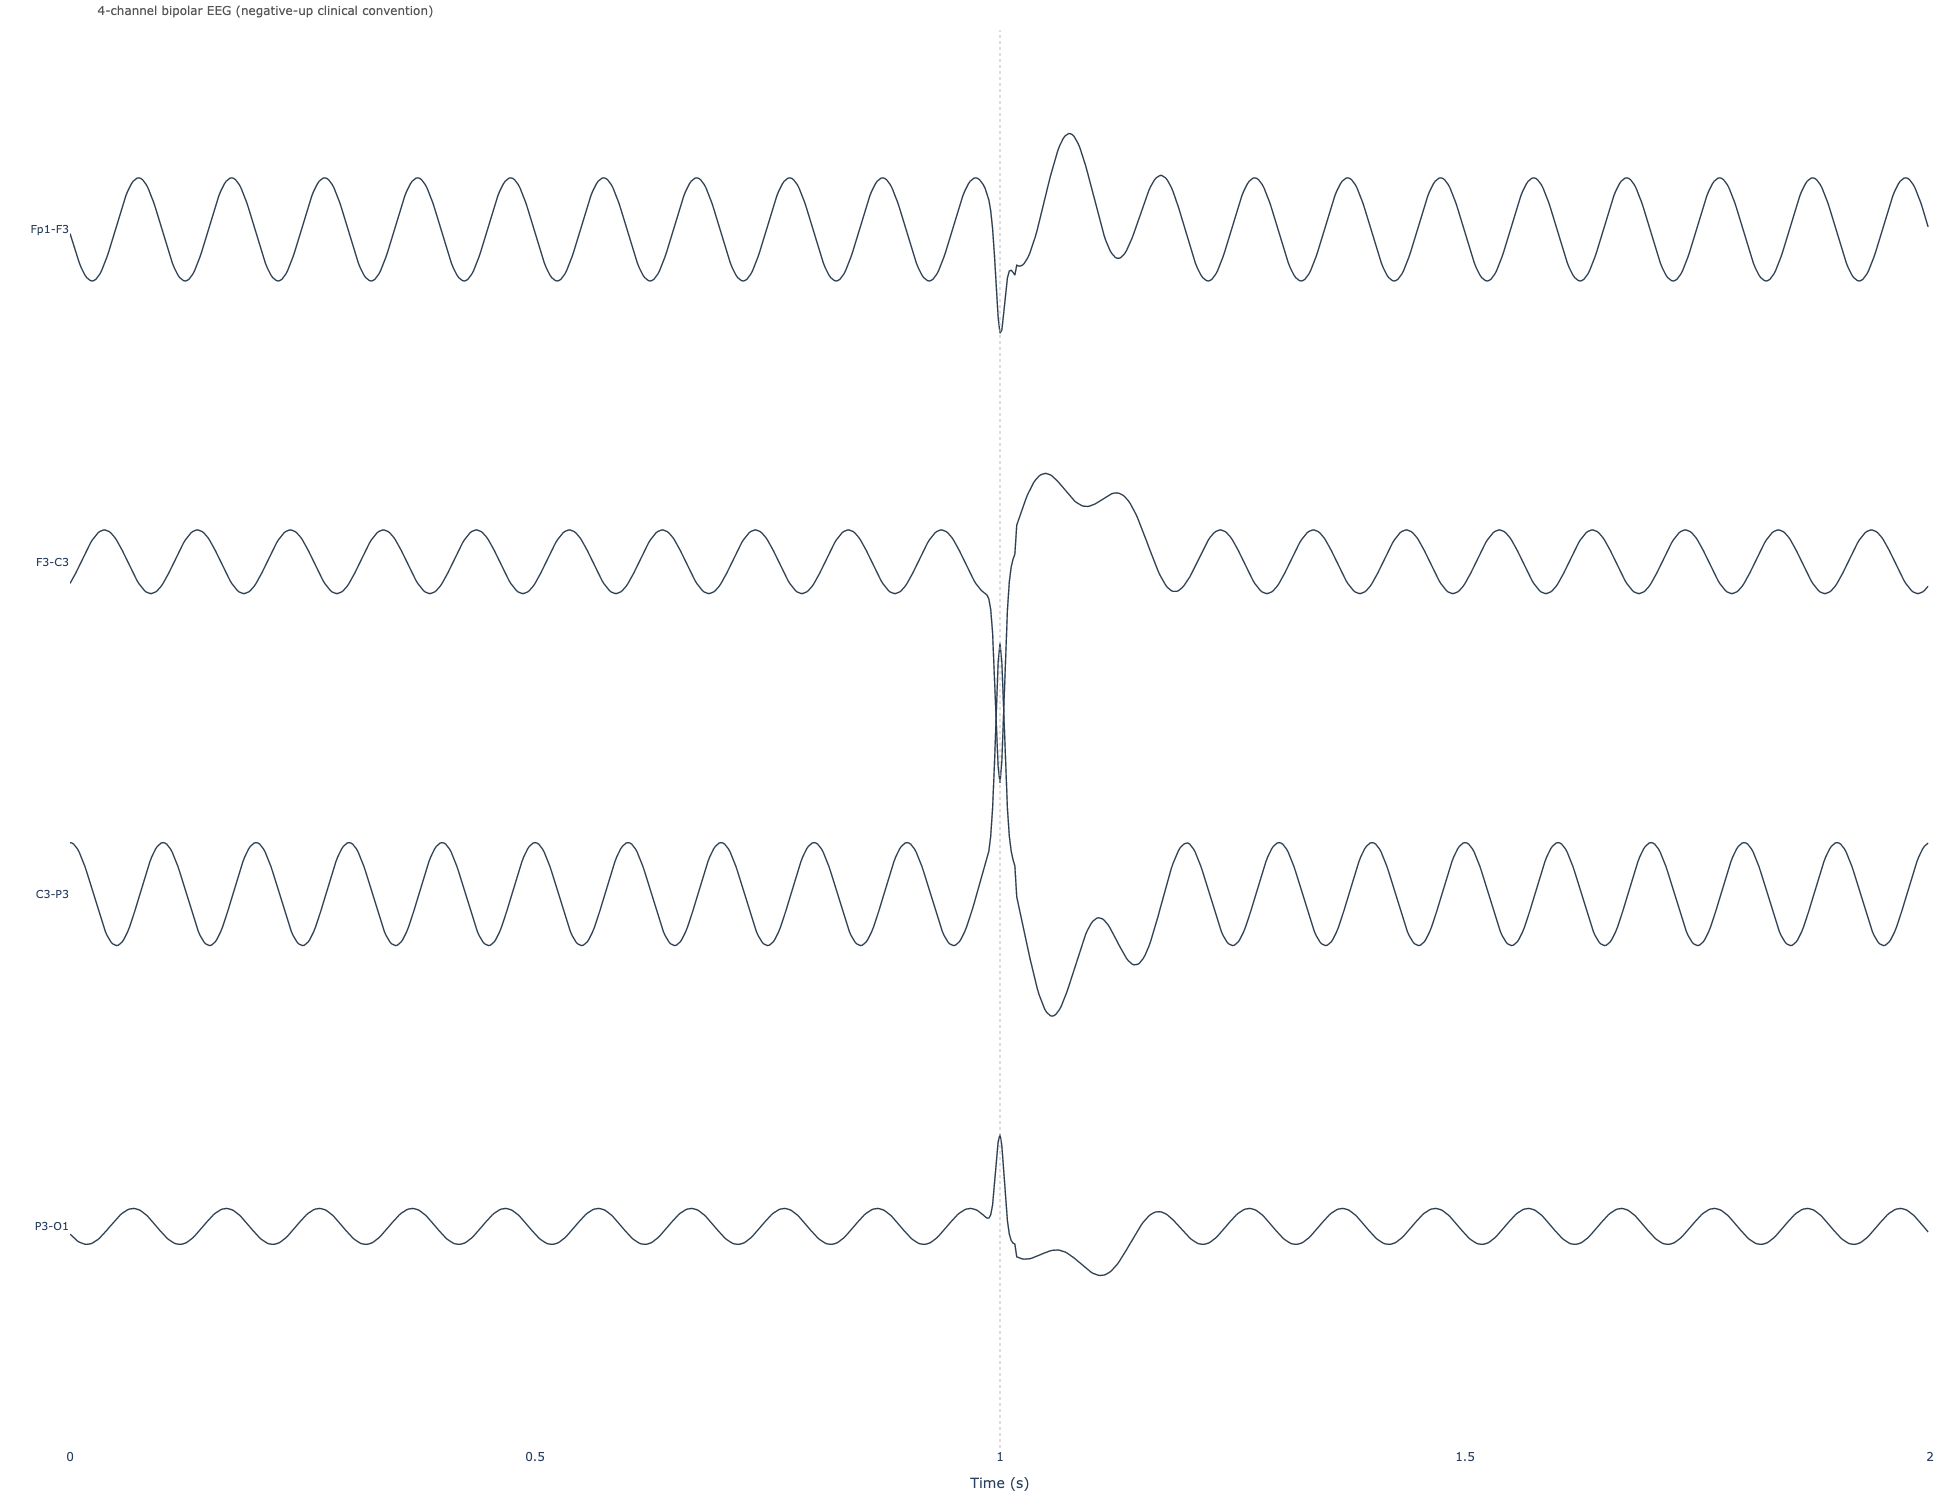
\includegraphics[width=0.85\textwidth]{figures/prob6_phase_reversal.png}
\end{center}

\textit{(a) Electrode closest to the source? (b) How can you tell?}

\answer{(a) \textbf{C3}.
\\(b) The two channels that share C3 --- \textbf{F3-C3} and \textbf{C3-P3} --- deflect in opposite directions at the spike (one downward, one upward). This is a \textbf{phase reversal}. The shared electrode of a phase reversal points to the source.}
\why{In a bipolar montage each channel is the difference $V_A - V_B$. A focal source under one electrode produces opposite-sign contributions in any pair of channels that include it.}

% ──────────────────────────────────────────────────────────────────────
\section*{Problem 8 — The Double Banana}
\textit{(a) List the four electrode chains of the longitudinal bipolar (double banana) montage. (b) What kind of brain activity does this montage tend to underestimate?}

\answer{(a) Four front-to-back chains:
\begin{itemize}[leftmargin=*,nosep]
\item \textbf{Left parasagittal:} Fp1 $\to$ F3 $\to$ C3 $\to$ P3 $\to$ O1
\item \textbf{Right parasagittal:} Fp2 $\to$ F4 $\to$ C4 $\to$ P4 $\to$ O2
\item \textbf{Left temporal:} Fp1 $\to$ F7 $\to$ T3 $\to$ T5 $\to$ O1
\item \textbf{Right temporal:} Fp2 $\to$ F8 $\to$ T4 $\to$ T6 $\to$ O2
\end{itemize}
(b) \textbf{Lateral / inter-hemispheric activity} --- differences between left and right at the same anterior-posterior level. Because all four chains run front-to-back, side-to-side voltage differences never appear as a phase reversal; they smear across the chain instead. The \textbf{transverse bipolar montage} (left-to-right chains) is used to catch this.}
\why{Each chain only sees voltage gradients along its own direction. A purely lateral asymmetry has no front-to-back gradient, so the double banana under-represents it. Different montages reveal different patterns --- which is why neurologists switch montages while reading.}

% ──────────────────────────────────────────────────────────────────────
\section*{Problem 9 — Artifacts}

\begin{center}
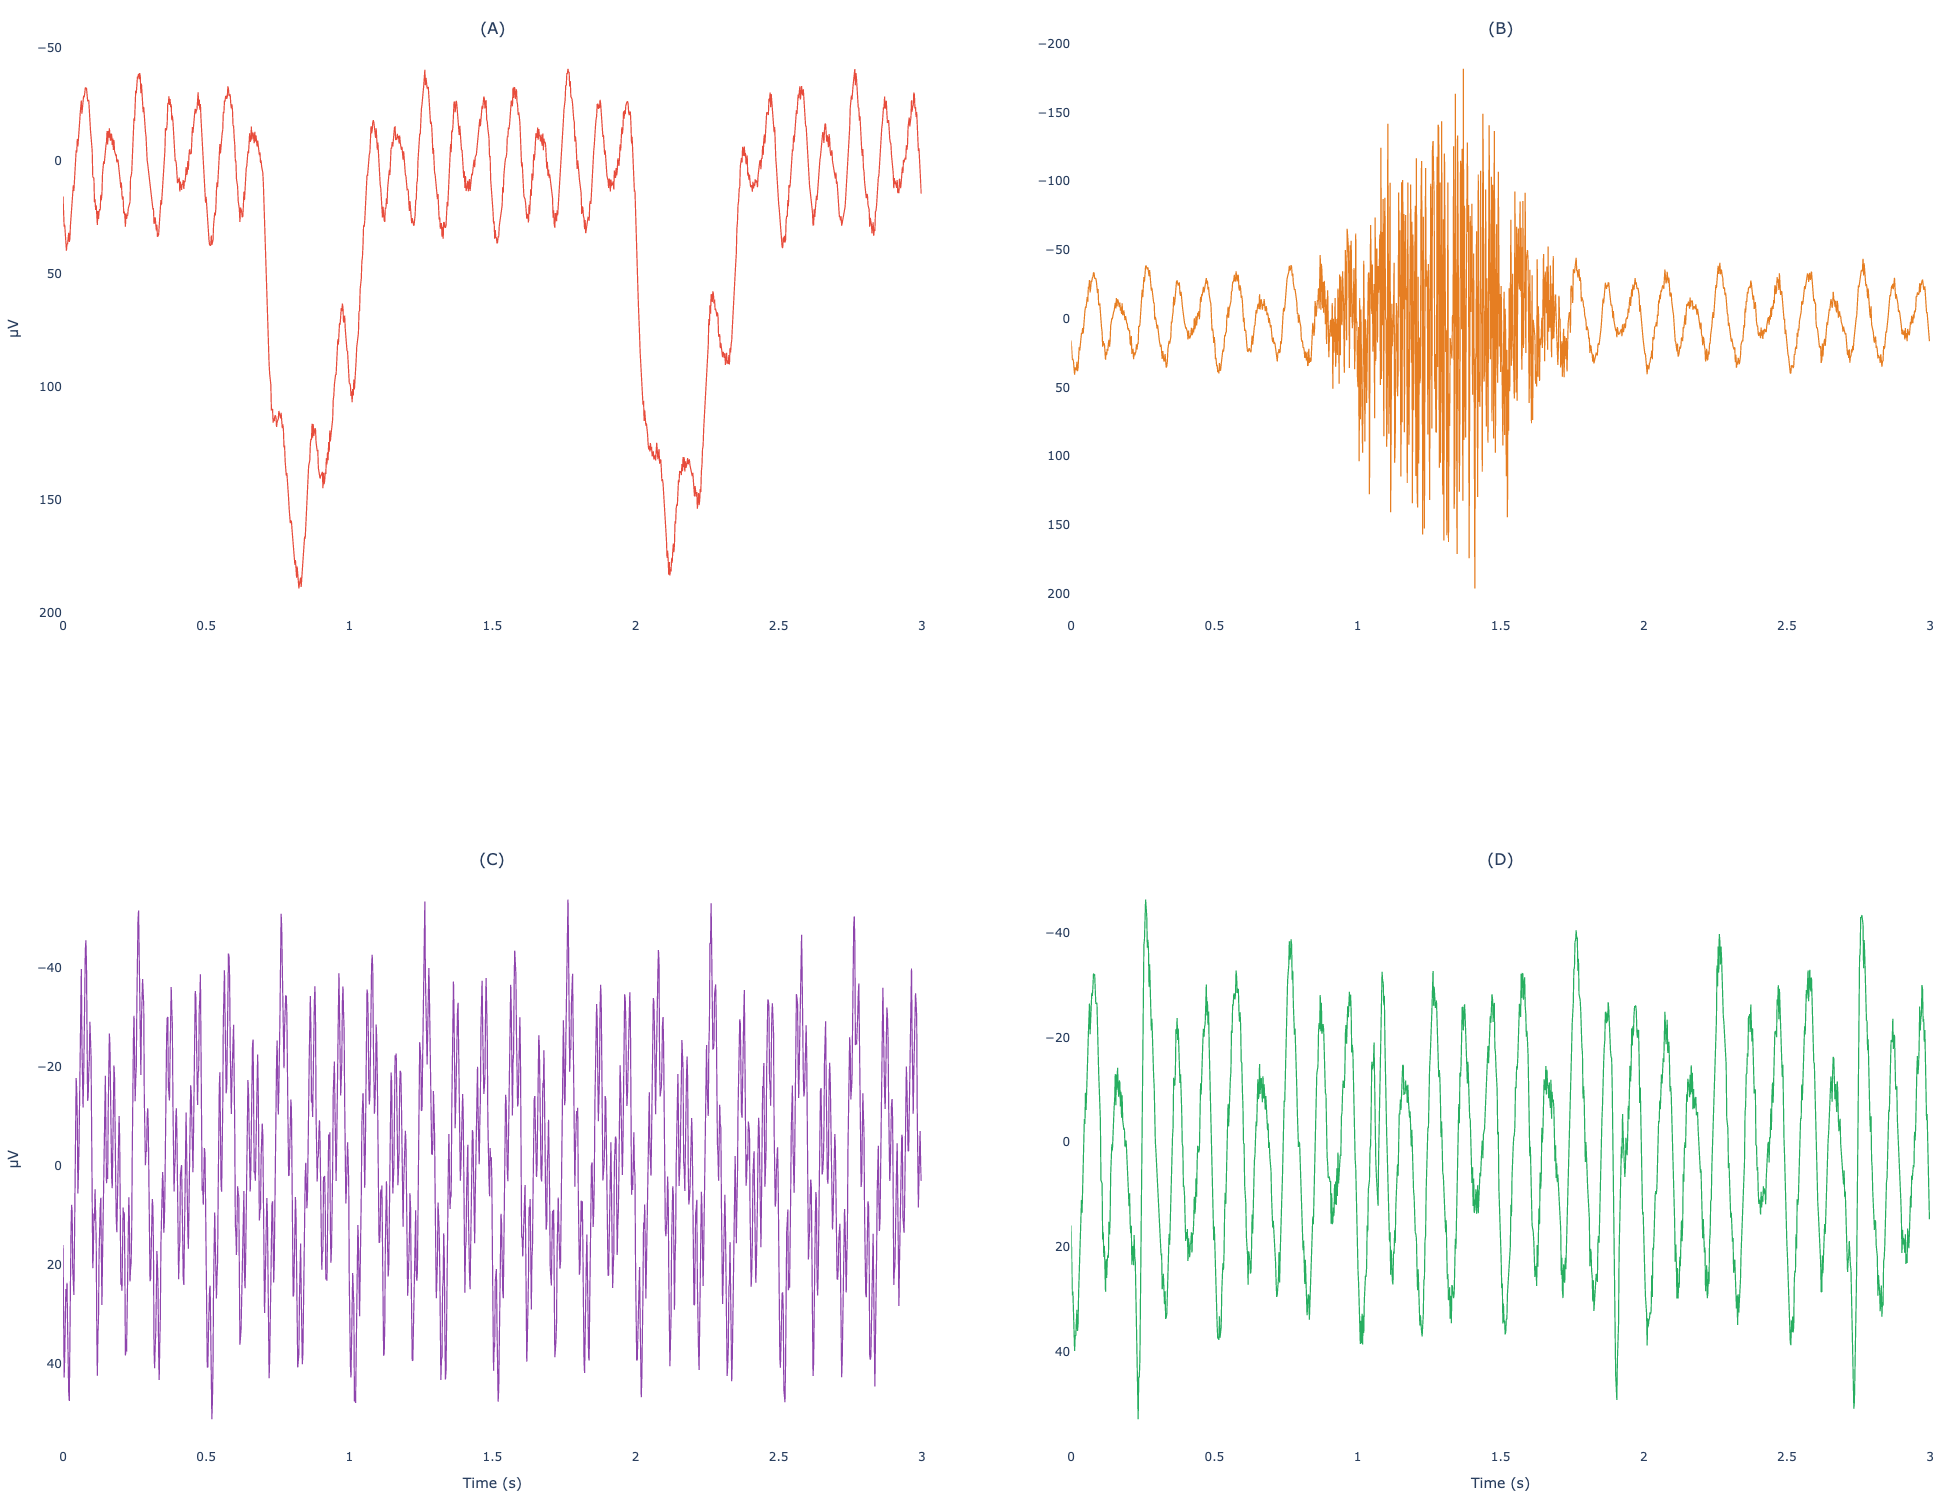
\includegraphics[width=0.85\textwidth]{figures/prob7_artifact_grid.png}
\end{center}

\textit{Identify each panel; pick one and give a removal strategy.}

\answer{
\begin{tabular}{ll}
\textbf{Panel} & \textbf{Artifact} \\
\hline
\rule{0pt}{1.1em} A & \textbf{Eye blink} --- large slow asymmetric deflection \\
B & \textbf{Muscle (EMG)} --- high-frequency broadband fuzz, burst-like \\
C & \textbf{60\,Hz line noise} --- perfectly regular, dense sinusoid \\
D & \textbf{ECG (cardiac)} --- sharp periodic spikes at $\sim$1.2\,Hz \\
\hline
\end{tabular}

\vspace{0.5em}
\textbf{Removal} (any one is sufficient):
\begin{itemize}[leftmargin=*,nosep]
\item \textit{Blink:} Independent Component Analysis (ICA) to subtract the blink component, or ask the patient to fixate on a point.
\item \textit{Muscle:} Ask the patient to relax the jaw and face; low-pass filter (caveat: loses real high-frequency brain activity).
\item \textit{60\,Hz:} Notch filter centered at 60\,Hz; check electrode impedances.
\item \textit{ECG:} Record a simultaneous ECG channel and subtract its projection.
\end{itemize}}
\why{Each artifact has a distinctive morphology and spectral signature. Recognizing them is the first step --- only then can you remove them or reject the contaminated epoch.}

% ──────────────────────────────────────────────────────────────────────
\section*{Problem 10 — Spectrograms}
\textit{Window 0.5\,s vs 2\,s: (a) what improves vs worsens? (b) which for seizure-onset detection?}

\answer{(a) Going 0.5\,s $\to$ 2\,s:
\begin{itemize}[leftmargin=*,nosep]
\item Frequency resolution \textbf{improves} (sharper). $\Delta f = 1/T$, so it goes from $1/0.5 = 2$\,Hz down to $1/2 = 0.5$\,Hz.
\item Time resolution \textbf{worsens}. Each time slice now covers 2\,s instead of 0.5\,s, so events are smeared horizontally.
\end{itemize}
(b) Use the \textbf{shorter (0.5\,s) window}. Seizure onset must be localized to within a fraction of a second; you accept coarser frequency precision in exchange for sharp temporal precision.}
\why{Time--frequency uncertainty: $\Delta f = 1/T$. You cannot simultaneously have fine frequency resolution and fine time resolution. Sharp temporal events demand short windows; slow-rhythm characterization (sleep staging) tolerates long windows.}

% ──────────────────────────────────────────────────────────────────────
\section*{Problem 11 — The Real Thing (Module 8)}
\textit{Load \texttt{chb03\_01.edf} from the CHB-MIT Scalp EEG Database. Answer five questions.}

\answer{(a) \textbf{23 channels.} Sampling rate: \textbf{256\,Hz.} Duration: $\sim$\textbf{51.1 minutes} (3068 seconds).

\textit{Note:} The EDF header says 3600\,s but the actual recording is shorter.

\medskip
(b) \textbf{Bipolar montage.} The channel names are electrode pairs (e.g., FP1-F7, F7-T7, T7-P7), not individual electrodes. Each channel is the voltage difference between two adjacent electrodes.

\medskip
(c) Seizure onset at approximately \textbf{362 seconds}, ending at approximately \textbf{414 seconds}. Duration: $\sim$\textbf{52 seconds}.

\medskip
(d) See verification plot below.

\begin{center}
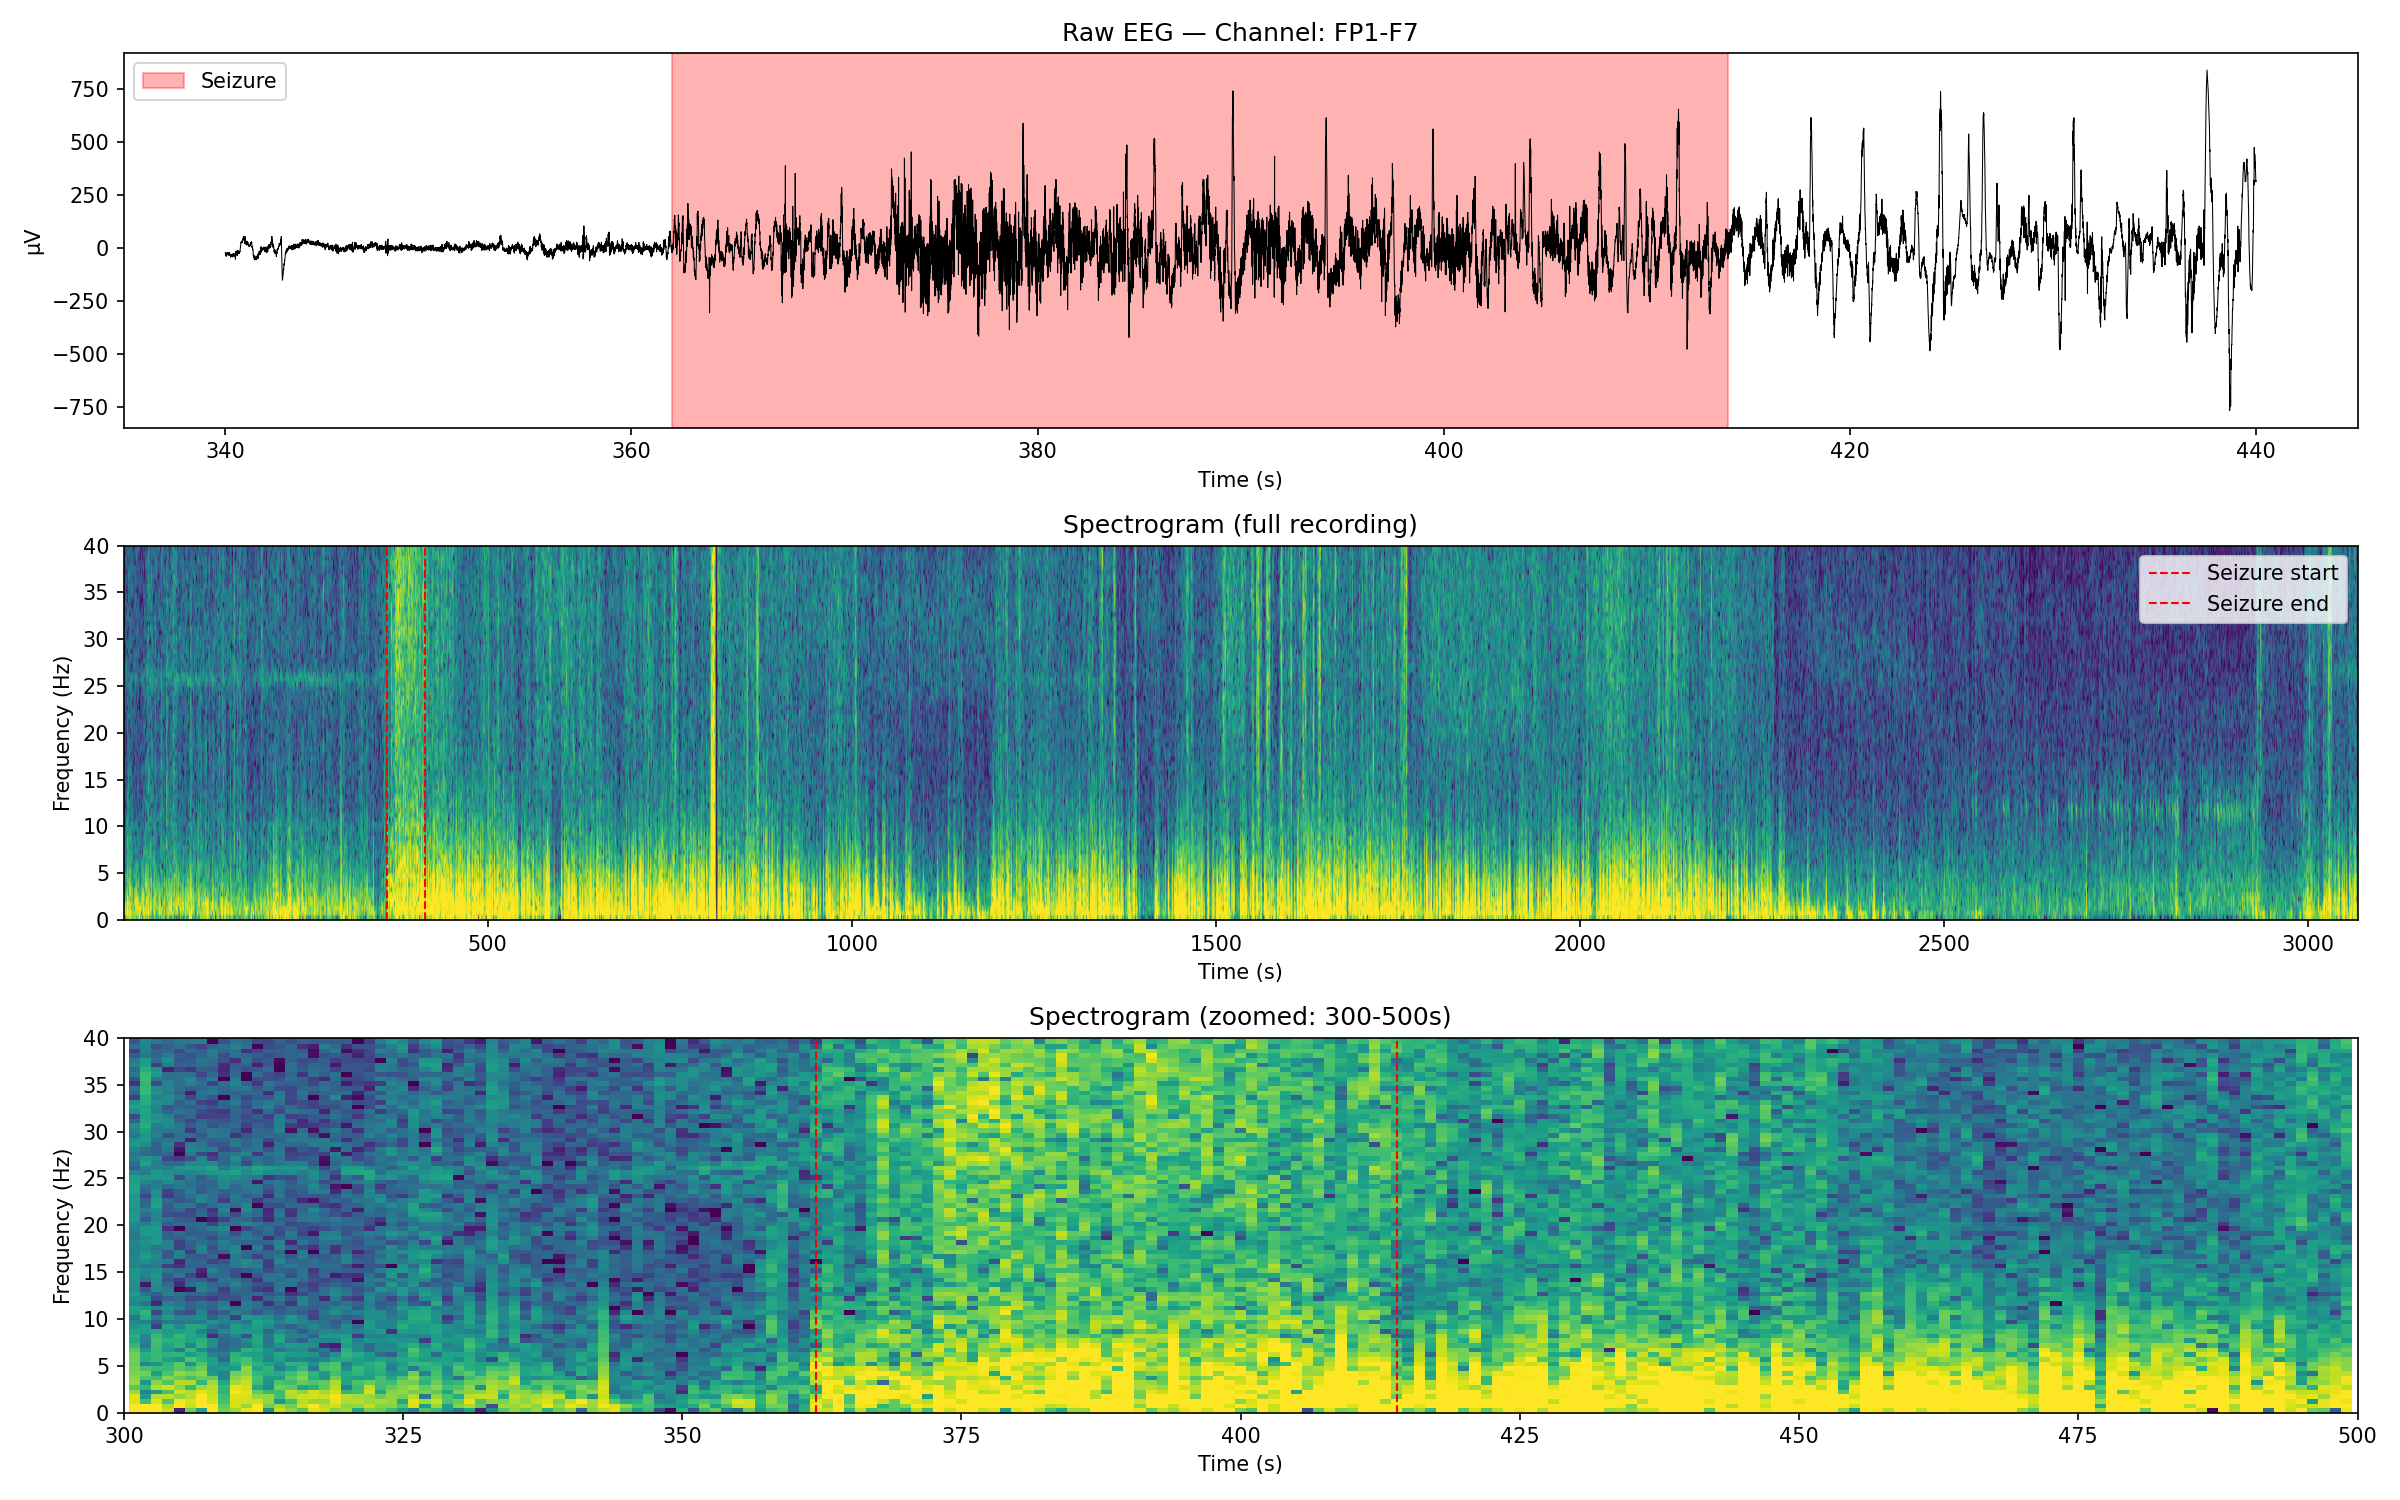
\includegraphics[width=\textwidth]{../assets/eeg_data/verification_plot.png}
\end{center}

The spectrogram shows a sudden broadband power increase starting at $\sim$362\,s, spanning 0--40\,Hz, lasting about 52 seconds. This is consistent with electrographic seizure activity.

\medskip
(e) The patient is having an \textbf{electrographic seizure}. The EEG shows sudden onset of rhythmic activity with broadband power increase at 362 seconds, lasting 52 seconds. Combined with the clinical history of staring spells with lip-smacking, this is consistent with \textbf{focal seizures} (likely temporal lobe epilepsy).}

\why{The CHB-MIT dataset annotates this seizure at 362--414\,s. The spectrogram makes it obvious: a clear transition from normal background to broadband rhythmic activity, then gradual post-ictal slowing. The bipolar montage is identifiable from channel names alone --- no metadata lookup required.}

\end{document}
